% !TeX root = Report.tex
\section{Predicate Evaluation}

\subsection{Predicate Scripting Language}

\subsubsection{Required Features}

\begin{enumerate}
	\item Numerical support (Integer and Floating point) ($+$ $-$ $\times$ $/$ $=$ $\neq$ $<$ $\leq$ $>$ $\geq$)
	\item Set support (Creation and operating on) ($\cup$ $\cap$ $\setminus$ $\{\}$ $\forall$ $\exists$)
	\item Limited function support (eg. $Neighbourhood(N, H)$)
	\item Limited struct support (eg. $N.Temperature$)
	\item Ability to specify predicate target(s) (Single node, multiple nodes or entire network)
	\item Ability to get the current node ($this$)
	\item Ability to get sensor information on a node (temperature, humidity, \ldots)
	\item Ability to get node information (Distance to Sink, \ldots)
\end{enumerate}

\subsubsection{Non-Required Features}

There are lots of features that are usually provided by scripting languages that would cause undesirable effects such as inflating the binary size.

\begin{enumerate}
	\item Strings
	\item Complicated data structures (Lists, Arrays, Dictionaries, \ldots)
	\item Library features (Custom libraries or built-in libraries)
	\item Interactive mode (terminals)
	\item IO
\end{enumerate}


\subsubsection{Evaluation Methods}

\begin{enumerate}
	\item Send scripting language to node, they interpret and evaluate it
	\item Compile predicate on base station, compress and send to node(s) for evaluation
\end{enumerate}

\subsubsection{Scripting Languages Considered}

\begin{enumerate}
	\item eLua \url{http://www.eluaproject.net/} \cite{elua}
	\item SCript \url{http://www.sics.se/~adam/dunkels06lowoverhead.pdf} \cite{dunkels06lowoverhead}
	\item wren \url{https://github.com/darius/wren} \cite{wren}
	\item Write the predicate in C, compile it to machine code and send it to the nodes to be evaluated
	\item \url{http://dunkels.com/adam/tsiftes11database.pdf} Antelope
\end{enumerate}


\subsubsection{Getting and Waiting for Neighbourhood Data}

\begin{enumerate}
	\item If all neighbours are known then 1-hop predicates can wait for each node to send data. This has extra memory and communication requirements
	\item If we do not know who our n-hop neighbours are then we can just set a time out to wait for results
	\begin{enumerate}
		\item If we do not receive all items what should be done?
		\item Should we report that the predicate is true, even though we didn't receive all the information?
	\end{enumerate}
	\item What data should be sent from surrounding nodes and how could we access it?
\end{enumerate}



\subsection{Where to Evaluate Predicates}

Given the problem of assigning slots in a TDMA MAC protocol, one would wish to ensure that no node within two hops of any given node has the same slot. This raises a question of where this predicate should be evaluated to ensure minimum energy usage in its evaluation.

The first predicate we might consider is the one where for ever node, we get the 2-hop neighbourhood and check that none of those nodes have the same slot as the initial node. This means that we would need to send:
\begin{enumerate}
	\item A message from the base station to the node asking it to evaluate the predicate
	\item A message from the node to each of its 2-hop neighbours
	\item Each 2-hop neighbour needs to send a message back to the node
	\item The node would need to wait for its neighbours to send the messages, then evaluate the predicate. This would imply that the node would need to know who is in its two hop neighbourhood
	\item The node would need to report to the base station the result of the predicate
\end{enumerate}

So we would need at best $2\Delta_{sink} + 2|Neighbours(n, 2)|$ messages to evaluate this predicate for one node.

\begin{align}
\label{eq:2-hop-slot-pred}
& \hspace{3em}	\forall n \in Nodes \cdot \\
& \hspace{6em}		\forall n' \in Neighbours(n, 2) \cdot \\
& \hspace{9em}			(n.slot \neq n'.slot)
\end{align}


The second predicate we could consider is the one where every node checks their 1-hop neighbourhood for slot collisions. Here we model the 2-hop nature of the predicate differently, because instead of checking on the node that we want to check for slot collisions, we check on the node between two nodes that might have slot collisions.

\begin{enumerate}
	\item A message from the base station to the node adjacent to that we asking to check slot collisions
	\item A message from the node to each of its 1-hop neighbours
	\item Each 1-hop neighbour needs to send a message back to the node
	\item The node would need to wait for its neighbours to send the messages, then evaluate the predicate. This would imply that the node would need to know who is in its two hop neighbourhood
	\item The node would need to report to the base station the result of the predicate
\end{enumerate}

So we would need at best $2(\Delta_{sink} + 1) + 2|Neighbours(n, 1)|$ messages to evaluate this predicate for one node.

\begin{align}
\label{eq:1-hop-slot-pred}
&				\forall n \in Nodes \cdot \\
& \hspace{3em}		\forall n' \in Neighbours(n, 1) \cup \{n\} \cdot \\
& \hspace{6em}			\forall n'' \in Neighbours(n, 1) \cup \{n\} \cdot \\
& \hspace{9em}				(n' \not= n'' \implies n'.slot \neq n''.slot)
\end{align}

Overall we can assume that $|Neighbours(1, n)| \leq |Neighbours(2, n)|$, so checking 1-hop neighbours would in general require fewer message. Also we can assume that when checking these predicates, we would make sure that every node is checked (as the predicates are defined). This means that the first predicate would duplicate the checks: checking node $n$ for a collision with $n'$ and when $n'$ is asked to check the predicate it will query $n$.

However, if we were not asking the entire network to check for this property, then the first predicate would behave better. This is because the second predicate would have to be called for every 1-hop neighbour of the intended node. However, as it is assumed that the entire network would be asked if this predicate holds, then the second predicate is better.


\subsection{Implementing Primitives}

There are certain primitives that we are going to need to implement. One of these is the $Neighbours(n, h)$ primitive, that takes a parameter $n$ that is the node we wish to get neighbour information on and $d$ which is the distance in hops from the node $n$ that we will ask for information.

\begin{align}
\label{eq:hcluster-neighbours-predicate}
& \hspace{3em}	\forall n \in Nodes \cdot \\
& \hspace{6em}		\exists n' \in Neighbours(n, H) \cdot \\
& \hspace{9em}			IsClusterHead(n)
\end{align}

An example of a predicate that uses $Neighbours(n, h)$ is shown above. This predicate is for Hierarchical Clustering where $H$ is a parameter that defines the distance between cluster heads. The predicate checks that for every node there is a neighbour in the $H$-hop neighbourhood that is a cluster head.

An alternative way that we might specify this predicate is to check that the distance between a node and the cluster head (that it knows the address of) is within $H$ hops.

\begin{align}
\label{eq:hcluster-distance-predicate}
& \hspace{3em}	\forall n \in Nodes \cdot \\
& \hspace{6em}		IsSink(n) \lor Distance(n, ClusterHead(n)) \leq H
\end{align}

However, there is an issue with this predicate. How would we implement the $Distance(n, n')$ primitive? With $Neighbours(n, h)$ we know how far we need to ask for information ($h$ hops), with $Distance(n, n')$ the maximum distance that we will need to wait for information to return from is the diameter of the network. Unfortunately we cannot assume that the diameter is known. If instead we take a time-out approach there is no way that we can guarantee to wait for the correct amount of time. For example if we wait enough time to check if a node is at maximum $D$ hops from the given node the node will need to wait for $2 \times D \times T_{send}$ time units. However, if the node we are trying to find the distance of is at $D + 1 $ hops then we will not believe the two nodes are connected. To reliably wait to check if two nodes are connected in a network where the diameter is not known we will need to wait for $\infty$ time units. Thus making $Distance(n, n')$ impossible to implement without knowing the diameter.


\subsection{Domain Specific Language}

\subsubsection{Definition}
\begin{eqnarray*}
	\pn{eval} & \pp & [ \pn{target} ] \ww \pn{using} \\
	\pn{target} & \pp & \sm{all} \\
	~ & \oo & \pn{number}\sm{.}\pn{number} \\
%
	\pn{using} & \pp & \sm{using} \ww \sm{Neighbours}\sm{(}\pn{number}\sm{)} \ww \sm{as} \ww \pn{variable} \ww \sm{in} \ww \pn{using} \\
	~ & \oo & \pn{predicate} \\
%
	\pn{predicate} & \pp &  \sm{(}\pn{predicate}\sm{)} \\
	~ & \oo & \pn{quantifier}\sm{(}\pn{variable} \ww \sm{:} \ww \pn{variable} \ww \sm{\mytilde} \pn{predicate} \sm{)}\\
	~ & \oo &  \pn{predicate} \ww \pn{logical-binary} \ww \pn{predicate} \\
	~ & \oo &  \pn{logical-unary} \ww \pn{predicate} \\
	~ & \oo &  \pn{var-expr} \ww \pn{math-logical-binary} \ww \pn{var-expr} \\
%
	\pn{var-expr} & \pp & \sm{(}\pn{var-expr}\sm{)} \\
	~ & \oo & \pn{variable} \\
	~ & \oo & \pn{number} \\
	~ & \oo & \pn{string}\sm{(}\pn{this-variable}\sm{)} \\
	~ & \oo & \pn{var-expr} \ww \pn{math-binary} \ww \pn{var-expr} \\
	~ & \oo & \sm{abs}\sm{(}\pn{var-expr}\sm{)} \\
	~ & \oo & \pn{set-fn}\sm{(}\pn{variable}\sm{)} \\
	~ & \oo & \pn{transform-set-fn}\sm{(}\pn{transform-fn}\sm{,} \ww \pn{variable}\sm{)} \\
%
	\pn{this-variable} & \pp & \pn{variable} \oo \sm{this} \\
	\pn{variable} & \pp & \pn{string} \\
%
	\pn{transform-fn} & \pp & \pn{string} \\
	\pn{transform-set-fn} & \pp & \sm{sum} \oo  \sm{mean} \oo \sm{max} \oo \sm{min} \\
	\pn{set-fn} & \pp & \sm{len} \\
%
	\pn{logical-binary} & \pp & \sm{\&}  \oo \sm{\textbar} \oo \sm{\textasciicircum} \oo \sm{=\textgreater} \oo \sm{\textless=\textgreater} \\
	\pn{logical-unary} & \pp & \sm{!} \\
	\pn{math-logical-binary} & \pp & \sm{==} \oo \sm{!=} \oo \sm{\textless} \oo \sm{\textless=} \oo \sm{\textgreater} \oo \sm{\textgreater=} \\
	\pn{math-binary} & \pp & \sm{+} \oo \sm{-} \oo \sm{*} \oo \sm{/} \oo \sm{**} \oo \sm{\%} \\
%
%	\pn{string} & \pp & \pn{alpha}\pn{string-rest} \\
%	\pn{string-rest} & \pp & \nn \oo \pn{alpha}\pn{string-rest} \oo \pn{digit}\pn{string-rest} \\
%
%	\pn{alpha} & \pp & \sm{A}\dots\sm{Z} \oo \sm{a}\dots\sm{z} \\
%	\pn{number} & \pp & \pn{sign} \pn{number-first} \oo \pn{number-first} \\
%	\pn{number-first} & \pp & \pn{digit} \oo \sm{1}\dots\sm{9}\pn{number-rest} \\
%	\pn{number-rest} & \pp & \pn{digit} \oo \pn{digit}\pn{number-rest} \\
%	\pn{digit} & \pp & \sm{0}\dots\sm{9} \\
%	\pn{sign} & \pp & \sm{+} \oo \sm{-} \oo \nn \\
	\pn{quantifier} & \pp & \sm{@} \oo \sm{\#} \\
\end{eqnarray*}

\textbf{TODO: Add float expansions}

used \url{http://cs.lmu.edu/~ray/notes/javacc/} and \url{http://www.engr.mun.ca/~theo/Misc/exp_parsing.htm} to get infix operator parsing working

\subsubsection{Examples}

\begin{figure}[H]
\begin{verbatim}
using Neighbours(2) as twohopn in
    @(x : twohopn ~
        slot(x) != slot(this)
    )
\end{verbatim}
\caption{Check that no two neighbours have the same slot}
\end{figure}

\begin{figure}[H]
\begin{verbatim}
using Neighbours(1) as onehopn in
    @(x : onehopn ~
        @(y : onehopn ~
            addr(x) != addr(y) => slot(x) != slot(y)
        )
    )
\end{verbatim}
\caption{Check that no two neighbours have the same slot \cite{DBLP:journals/corr/abs-0808-0920}}
\end{figure}

\begin{figure}[H]
\begin{verbatim}
temperature(this) <= 40.0
\end{verbatim}
\caption{Check that our temperature is less than or equal to 40 degrees}
\end{figure}

\begin{figure}[H]
\begin{verbatim}
using Neighbours(2) as twohopn in
    abs(temperature(this) - mean(temperature, twohopn)) <= 10.0
\end{verbatim}
\caption{Check that the average neighbour temperature is with 10 degrees of ours}
\end{figure}


\begin{figure}[H]
\begin{verbatim}
using Neighbours(H(this)) as neighbours in
    #(node : neighbours ~
        ch(this) == addr(node)
    )
\end{verbatim}
\caption{Check cluster head is in H-hop neighbourhood}
\end{figure}



\begin{figure}[H]
\begin{verbatim}
using Neighbours(1) as onehopn in
    using Neighbours(2) as twohopn in
        @(a : onehopn ~
            #(b : twohopn ~ addr(a) == addr(b))
        )
\end{verbatim}
\caption{Check 1-hop neighbourhood is in 2-hop neighbourhood}
\end{figure}


\begin{figure}[H]
\begin{verbatim}
using Neighbours(1) as onehopn in
    base-station-distance(this) == min(base-station-distance, onehopn) + 1
\end{verbatim}
\caption{We are one hop further from the base station than the closest of our neighbours}
\end{figure}


\subsection{Virtual Machine}

\subsubsection{Opcodes}

\begin{verbatim}
_ is either I for int or F for float

For binary operations the order the operands are used is specified as x op x.
When x is 0 the value on the top of the stack is used. When x is 1 the
value after the one on the top of the stack is used.

HALT
    Halts execution.
    The stack should always have at least one integer on it when halting.

_PUSH (_)
    Pushes an _ onto the stack.

_POP
    Pops the stack by sizeof(_) bytes.

_FETCH (variable id - ubyte)
    Fetches the value of the given variable and pushes the
    first sizeof(_) bytes of it onto the stack.

_STORE (variable id - ubyte)
    Stores the first sizeof(_) bytes in the variable
    of the given name.

AFETCH (variable id - ubyte)
    Fetches the value of the array named in the parameter
    at the integer index at the top of the stack.

ALEN (variable id - ubyte)
    Pushes an integer onto the stack containing the length
    of the named array.
	
ASUM  (variable id - ubyte) (function id - ubyte)
AMEAN
AMAX
AMIN
    Over the user defined array stored in the variable whose
    name is the first parameter, transform it using the function
    whose name is the second parameter. On this transformed data
    calculate the array operation and push the result as a float
    onto the top of the stack.

CALL (function id - ubyte)
    Calls the named function on the data on top of the stack.
    Pop's the data that was given to the function off the top of
    the stack and pushes the result onto the top of the stack.

ICASTF
    Pops an integer off the stack, casts it to a float
    then stores it back on the stack.

FCASTI
    Pops a float off the stack, casts it to a integer
    then stores it back on the stack.

JMP (ubyte)
    Jumps to a position in the code relative to the start
    of the program.

JZ (ubyte)
    Pops and reads the top of the stack as an integer, if it is 0
    the program jumps to the location, otherwise evaluation
    continues.

JNZ (ubyte)
    Pops and reads the top of the stack as an integer, if it is not 0
    the program jumps to the location, otherwise evaluation
    continues

_ADD        1 op 0
_SUB        1 op 0
_MUL        1 op 0
_DIV1       0 op 1
_DIV2       1 op 0
    Performs a mathematical operations on the first two sizeof(_)
    values on the stack. Pops both values off the stack, stores
    the result in the same type back on the stack.

IINC
    Pops the top of the stack by sizeof(int) bytes, increments
    the value as an integer. Pushes the result back on the stack

_EQ	        1 op 0
_NEQ        1 op 0
_ILT        1 op 0
_LEQ        1 op 0
_GT	        1 op 0
_GEQ        1 op 0
    Performs a mathematical operations on the first two sizeof(_)
    values on the stack. Pops both values off the stack, stores
    the result in an integer on the stack.

AND         1 op 0
OR          1 op 0
XOR	        1 op 0
EQUIVALENT  1 op 0
IMPLIES     1 op 0
    Performs a logical operation on the first two values on the
    stack. These are not bitwise operations and the expected
    formats of the values are integers. 0 is false, 1 is true.
    Pops both values off the stack,
    stores the result in an integer back on the stack.

NOT
    Pops an integer off the stack, performs logical not on it.
    Pushes the result back on the stack.
	
_VAR (variable id - ubyte)
    Creates a variable of type _ with the id set to the given
    unsigned byte.
\end{verbatim}


\subsubsection{Bytecode}

One of the most important aims of the predicate language's bytecode was to be as small as possible. The reason for this was to support sending as much program information in the limited length of a network packet. To achieve this aim it meant that we needed to make the virtual machine handle more abstract representations of its components. For example, initially the bytecode for calling a function contained a byte for the opcode of \verb|CALL| and then a string of characters which contained the name of the function to call. At minimum this would cost 2 bytes - one for the character of the function's name and one for the NUL character. To improve this the string was replaced with a single byte, which means that the number of functions callable by the virtual machine ends up being limited to 256. The same was true for the variable ids as well and as the variable id is contained with an unsigned byte, they to are limited to 256.


When developing the virtual machine what also became important was the fact that the bytecode was a string of unsigned bytes, where sequences of them could end up representing a 16 bit integer or a 32 bit float. This is important because it could mean that we would try to perform unaligned reads which the CPU of our motes could potentially get wrong\footnote{\url{http://permalink.gmane.org/gmane.os.contiki.devel/1462}}, this is due to the restrictions the CPU has on the alignment of words ``Bytes are located at even or odd addresses. Words are only located at even addresses \ldots. When using word instructions, only even addresses may be used. The low byte of a word is always an even address'' \cite[Section~1.4.5 (p.~28)]{msp430usersguide}.

\begin{figure}[ht!]
\centering
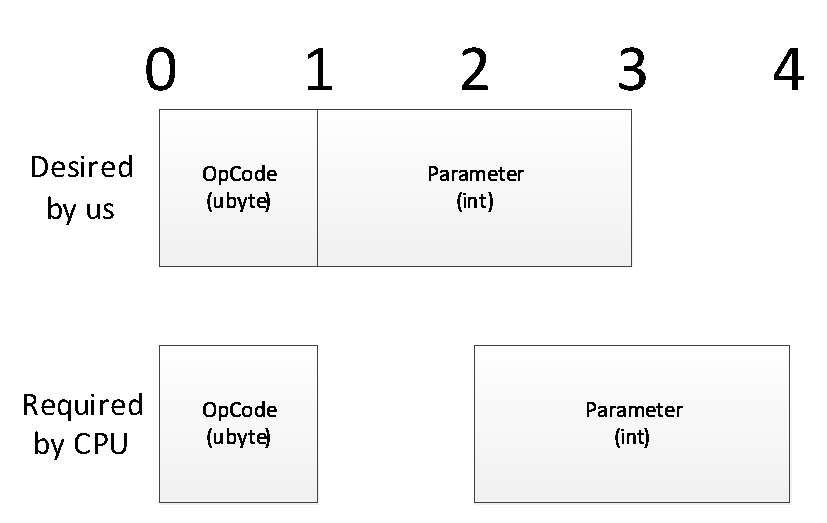
\includegraphics[scale=0.75]{Diagrams/byte-alignment.eps}
\caption{Alignment Issues}
\label{fig:alignment-issues}
\end{figure}

\begin{figure}[ht!]
\begin{verbatim}
[java] **** Illegal read - misaligned word from $2c01 at $80de
[java] Stack Trace: number of calls: 4 PC: $80de
[java] evaluate (errno.c) called from PC: $7166 (elapsed: 164446)
[java] process_thread_mainProcess (local in pred-eval.c) called from PC: $bf12 (elapsed: 536355)
[java] call_process (local in process.c) called from PC: $c0b2 (elapsed: 536391)
[java] process_run (errno.c) called from PC: $4250 (elapsed: 536996)
\end{verbatim}
\caption{Example of the error messages produced by MSPSim in Cooja that led to the discovery of this bug}
\end{figure}

As can be seen in \autoref{fig:alignment-issues} if we were to align the words as the CPU wanted the size of the bytecode would massively increase as every single byte bytecode would need to be padded by a byte to (i) make sure all bytecode entries were the same length and to ensure the word parameters are correctly aligned. To solve this issue instead of accessing the memory directly in the bytecode what can be done instead is to copy the memory out byte-by-byte into a correctly aligned block of memory and use that instead.


